% jupiter-c3-allinone.tex

% see https://tex.stackexchange.com/a/79925
\documentclass[varwidth]{standalone}

\usepackage{graphicx, subfigure}
    
\begin{document}
%%%%% fig:jupiter-c3-allinone %%%%%
\begin{figure}[t]
  \centering
  \subfigure[\textsl{AbsJupiter}]{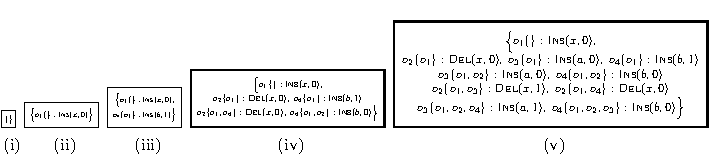
\includegraphics[width = 0.98\textwidth]{absjupiter-c3}}
  \subfigure[\textsl{CJupiter}]{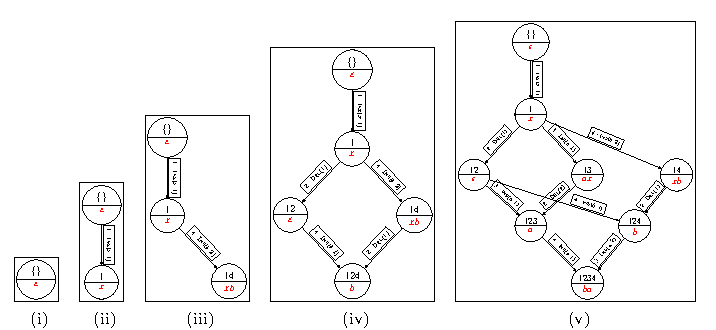
\includegraphics[width = 0.98\textwidth]{cjupiter-c3}}
  \subfigure[\textsl{XJupiter}]{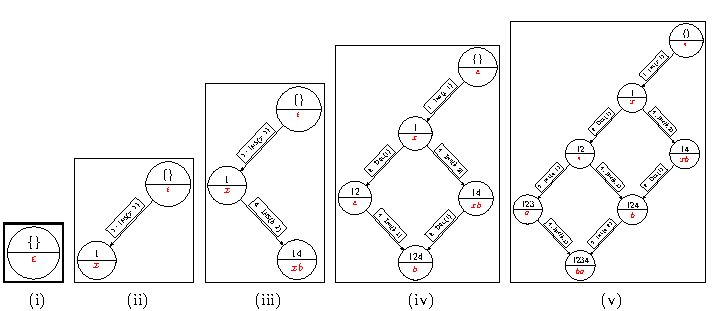
\includegraphics[width = 0.98\textwidth]{xjupiter-c3}}
  \subfigure[\textsl{AJupiter}]{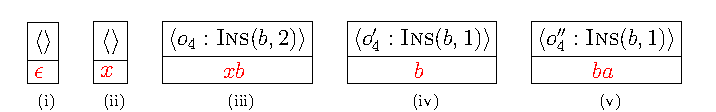
\includegraphics[width = 0.60\textwidth]{ajupiter-c3}}
\end{figure}
%%%%% fig:jupiter-c3-allinone %%%%%
\end{document}